\section{\textit{Exploratory Data Analysis} (EDA)}

Tahapan \textit{Exploratory Data Analysis} (EDA) bertujuan untuk mengenali karakteristik data dan mengidentifikasi pola hubungan di dalamnya sebelum diproses menggunakan algoritma pembelajaran mesin. Mengingat penelitian ini mengalami transisi dari penggunaan data sintetis (\textit{dummy}) menuju data operasional riil, tahapan EDA juga berperan penting dalam memvalidasi asumsi penelitian. Kemiripan maupun perbedaan pola yang ditemukan antara data sintetis dan data riil memberikan landasan empiris yang kuat, mengingat data sintetis tersebut sejak awal telah dirancang untuk merepresentasikan estimasi kondisi faktual penyewa di lapangan.

\subsection{Distribusi Kelas Target}
Pada tahap awal, distribusi kelas target disimulasikan menggunakan data sintetis dengan perbandingan penyewa Normal (Aman) berlabel 0 sebanyak 9.243 data, berbanding penyewa Tidak Normal (Melanggar) berlabel 1 sebanyak 746 data. Setelah sistem beroperasi, ekstraksi pada data riil memvalidasi proporsi ketimpangan tersebut, di mana diperoleh 453 data penyewa Normal dan 88 data penyewa Melanggar. Grafik perbandingan pada Gambar~\ref{fig:dist_kelas} memperlihatkan konsistensi ketimpangan jumlah data yang sangat besar (\textit{class imbalance}) pada kedua skenario. Kondisi ini dapat menyebabkan algoritma bias dan cenderung hanya memprediksi kelas mayoritas (penyewa normal). Oleh karena itu, ketimpangan ini wajib ditangani menggunakan sistem penalti pembobotan (\textit{cost-sensitive learning}) pada tahapan pelatihan model.

\begin{figure}[H]
    \centering
    \begin{subfigure}[b]{0.45\textwidth}
        \centering
        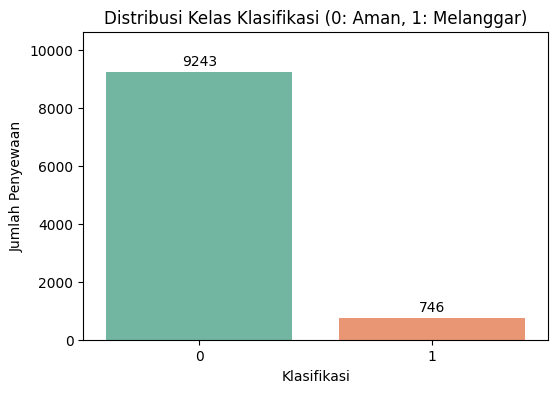
\includegraphics[width=\textwidth]{Gambar/Distribusi_Kelas_Dummy.png}
        \caption{Data Sintetis (\textit{Dummy})}
        \label{fig:dist_kelas_dummy}
    \end{subfigure}
    \hfill
    \begin{subfigure}[b]{0.45\textwidth}
        \centering
        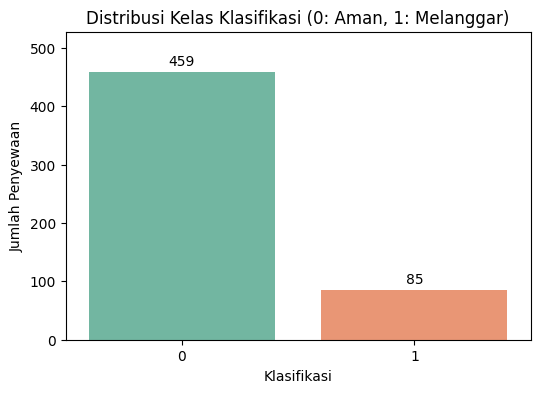
\includegraphics[width=\textwidth]{Gambar/Distribusi_Kelas_Riil.png}
        \caption{Data Riil}
        \label{fig:dist_kelas_riil}
    \end{subfigure}
    \caption{Perbandingan Distribusi Kelas Klasifikasi (0: Aman, 1: Melanggar)}
    \label{fig:dist_kelas}
\end{figure}

\subsection{Korelasi Antar Fitur Temporal (\textit{Heatmap})}
Analisis korelasi diterapkan pada fitur numerik untuk mengukur atribut yang paling berpengaruh terhadap label klasifikasi. Pada data sintetis, korelasi sengaja dibentuk berdasarkan hipotesis awal mengenai perilaku penyewa, di mana jam kedatangan (\textit{check-in}) dan lama menginap diasumsikan memiliki korelasi negatif terhadap label, masing-masing sebesar -0,24 dan -0,22. Hipotesis simulasi ini terbukti sangat relevan pada fitur lama menginap. \textit{Heatmap} data riil secara empiris justru mengonfirmasi keberadaan korelasi negatif yang melesat menjadi jauh lebih kuat, yakni mencapai -0,52 terhadap label pelanggaran. Peningkatan angka korelasi ini menegaskan bahwa semakin singkat durasi menginap seorang penyewa, semakin tinggi pula kemungkinan penyewa tersebut melakukan pelanggaran. 

Di sisi lain, terjadi perbedaan temuan pada variabel jam \textit{check-in}. Berbeda dengan asumsi sintetis yang memiliki korelasi -0,24, variabel jam kedatangan pada operasional riil sama sekali tidak menunjukkan korelasi (0,00) terhadap label. Penurunan drastis ini mengindikasikan adanya pergeseran pola di lapangan yang berbeda dari estimasi awal, di mana penyewa yang melanggar pada kondisi nyata tidak lagi memiliki kecenderungan kuat untuk datang pada jam-jam spesifik (seperti tengah malam), melainkan datang pada jam operasional yang wajar. Selain itu, pada data riil fitur seperti jenis sewa dan kewarganegaraan tidak memunculkan nilai korelasi karena seluruh transaksi riil murni berasal dari penyewa harian berkewarganegaraan WNI (tidak ada variansi data).

\begin{figure}[H]
    \centering
    \begin{subfigure}[b]{0.45\textwidth}
        \centering
        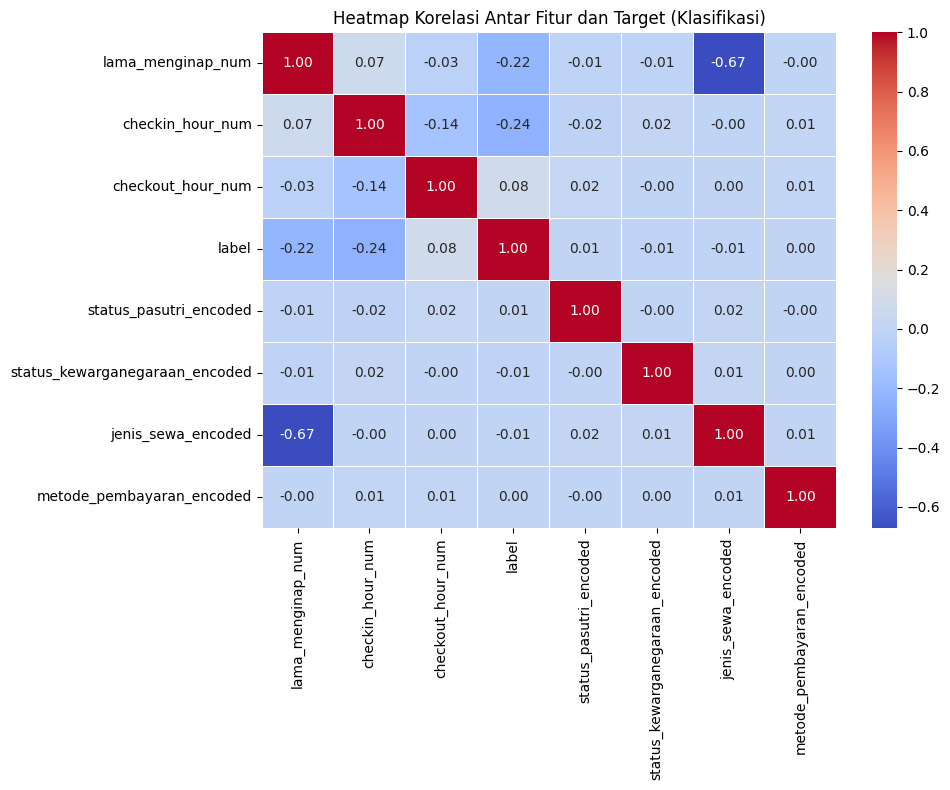
\includegraphics[width=\textwidth]{Gambar/Heatmap_Korelasi_Dummy.png}
        \caption{Data Sintetis (\textit{Dummy})}
        \label{fig:heatmap_korelasi_dummy}
    \end{subfigure}
    \hfill
    \begin{subfigure}[b]{0.45\textwidth}
        \centering
        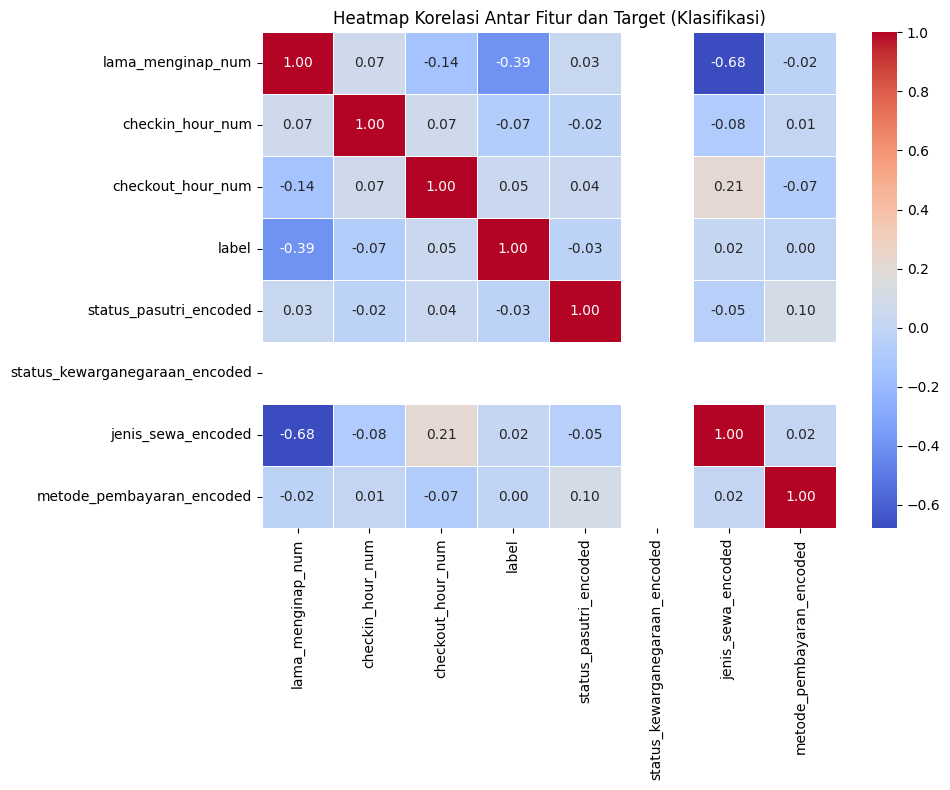
\includegraphics[width=\textwidth]{Gambar/Heatmap_Korelasi_Riil.png}
        \caption{Data Riil}
        \label{fig:heatmap_korelasi_riil}
    \end{subfigure}
    \caption{Heatmap Korelasi Antar Fitur dan Target}
    \label{fig:heatmap_korelasi}
\end{figure}

\subsection{Visualisasi Pola Penyewaan}
Tahap eksplorasi selanjutnya adalah membandingkan pola transaksi penyewa antara skenario simulasi dan kejadian nyata di lapangan.
\begin{enumerate}
    \item \textbf{Pola Jam \textit{Check-in}}\\ 
    Terdapat perbedaan temuan yang signifikan antara skenario simulasi dan operasional nyata. Pada data sintetis, asumsi awal menduga tingginya aktivitas kedatangan penyewa tidak normal terjadi secara spesifik pada jam-jam sepi (antara pukul 00:00 hingga 05:00 WIB). Namun, grafik pada Gambar~\ref{fig:pola_waktu} mengonfirmasi bahwa pada operasional riil di lapangan, seluruh aktivitas kedatangan penyewa (baik aman maupun melanggar) murni berpusat pada siang hingga malam hari, yakni di rentang pukul 13:00 hingga 20:00 WIB. Fakta ini menjelaskan bahwa pada kondisi nyata, pelanggaran tidak selalu terikat pada jam kedatangan yang tidak lazim.
    
    \begin{figure}[H]
        \centering
        \begin{subfigure}[b]{0.45\textwidth}
            \centering
            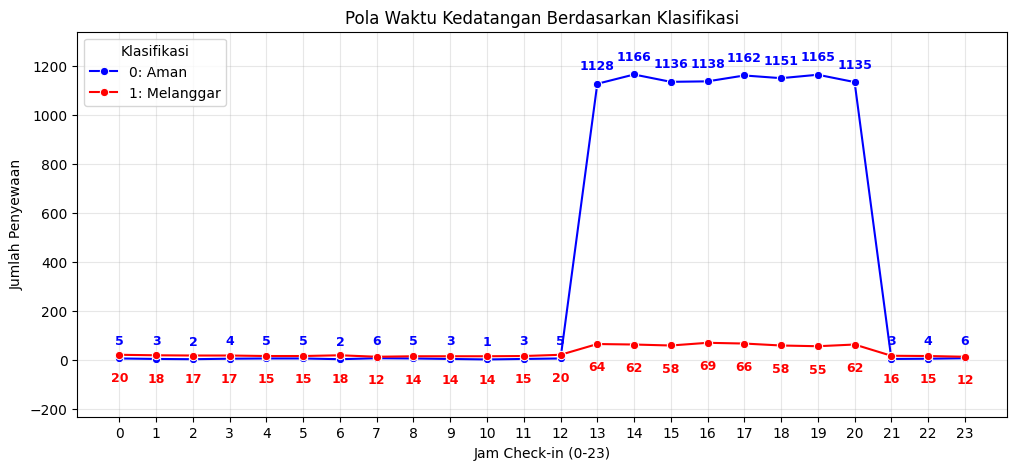
\includegraphics[width=\textwidth]{Gambar/Pola_Waktu_Kedatangan_Dummy.png}
            \caption{Data Sintetis (\textit{Dummy})}
            \label{fig:pola_waktu_dummy}
        \end{subfigure}
        \hfill
        \begin{subfigure}[b]{0.45\textwidth}
            \centering
            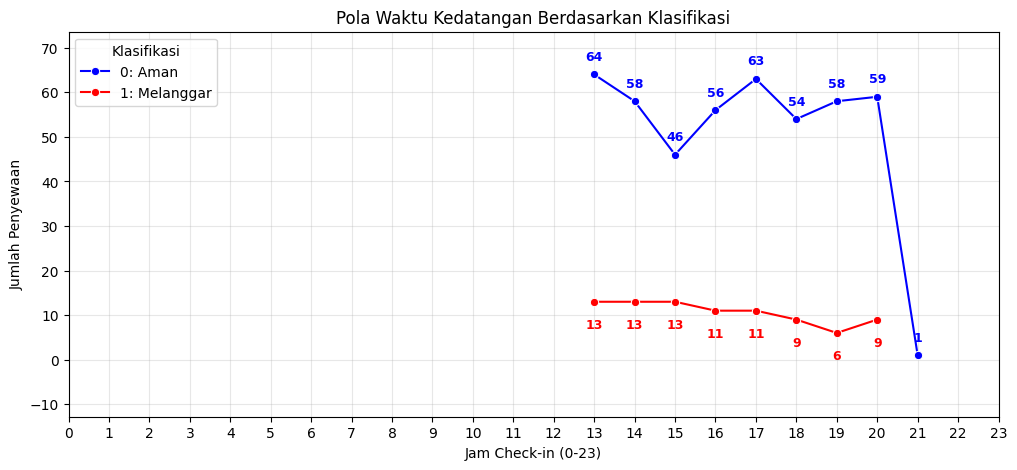
\includegraphics[width=\textwidth]{Gambar/Pola_Waktu_Kedatangan_Riil.png}
            \caption{Data Riil}
            \label{fig:pola_waktu_riil}
        \end{subfigure}
        \caption{Pola Waktu Kedatangan Berdasarkan Klasifikasi}
        \label{fig:pola_waktu}
    \end{figure}

    \item \textbf{Tren Lama Menginap}\\ 
    Sejalan dengan nilai korelasi kuat pada matriks sebelumnya, Gambar~\ref{fig:tren_menginap} membuktikan bahwa asumsi perancangan data sintetis sejalan dengan fakta di lapangan. Baik pada lingkungan simulasi maupun lingkungan nyata, kasus pelanggaran secara mutlak didominasi oleh penyewa dengan durasi inap yang sangat pendek. Pada data riil, 100\% kasus pelanggaran (88 kasus) terkonsentrasi hanya pada penyewa dengan lama inap 1 hari. Sebaliknya, penyewa dengan durasi inap jangka menengah hingga panjang terbukti memiliki profil yang sepenuhnya aman dari catatan pelanggaran.
    
    \begin{figure}[H]
        \centering
        \begin{subfigure}[b]{0.45\textwidth}
            \centering
            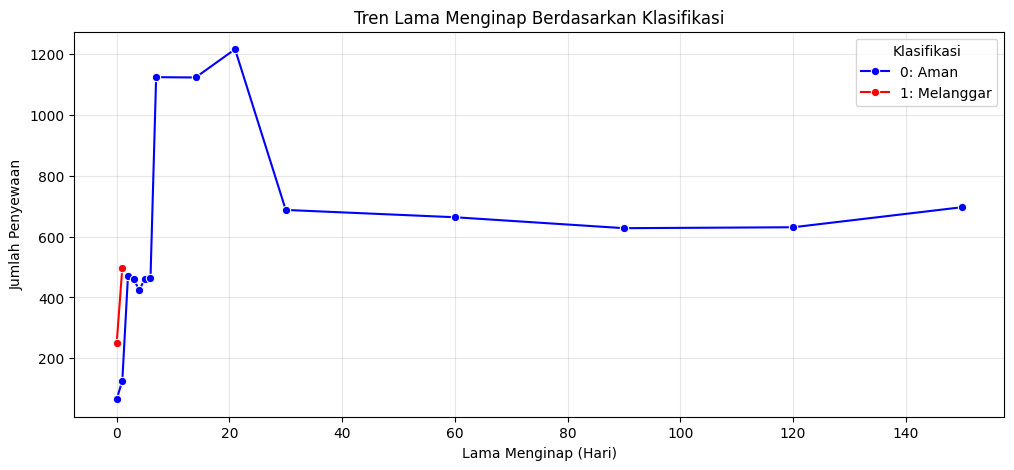
\includegraphics[width=\textwidth]{Gambar/Tren_Lama_Menginap_Dummy.png}
            \caption{Data Sintetis (\textit{Dummy})}
            \label{fig:tren_menginap_dummy}
        \end{subfigure}
        \hfill
        \begin{subfigure}[b]{0.45\textwidth}
            \centering
            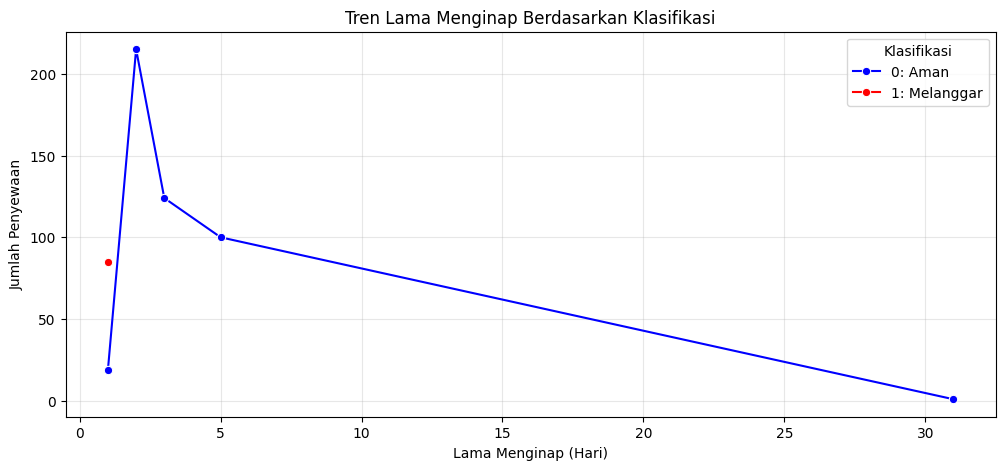
\includegraphics[width=\textwidth]{Gambar/Tren_Lama_Menginap_Riil.png}
            \caption{Data Riil}
            \label{fig:tren_menginap_riil}
        \end{subfigure}
        \caption{Tren Lama Menginap Berdasarkan Klasifikasi}
        \label{fig:tren_menginap}
    \end{figure}

    \item \textbf{Perbandingan Variabel Kategori}\\ 
    Berdasarkan Gambar~\ref{fig:jenis_sewa}, seluruh operasional nyata, termasuk 88 kasus pelanggaran murni didominasi oleh jenis sewa ``Harian''. Berbeda dengan data sintetis yang masih mensimulasikan penyewaan ``Mingguan'' dan ``Bulanan''. Perbedaan pola data operasional riil membuktikan bahwa asumsi simulasi sebelumnya mengenai tingginya risiko anomali yang hanya berpusat pada penyewa transit harian jangka pendek adalah benar.
    
    \begin{figure}[H]
        \centering
        \begin{subfigure}[b]{0.45\textwidth}
            \centering
            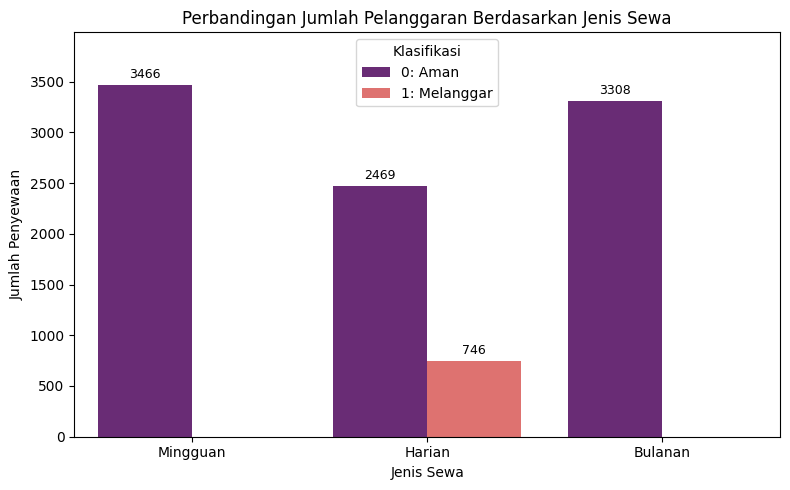
\includegraphics[width=\textwidth]{Gambar/Perbandingan_Jenis_Sewa_Dummy.png}
            \caption{Data Sintetis (\textit{Dummy})}
            \label{fig:jenis_sewa_dummy}
        \end{subfigure}
        \hfill
        \begin{subfigure}[b]{0.45\textwidth}
            \centering
            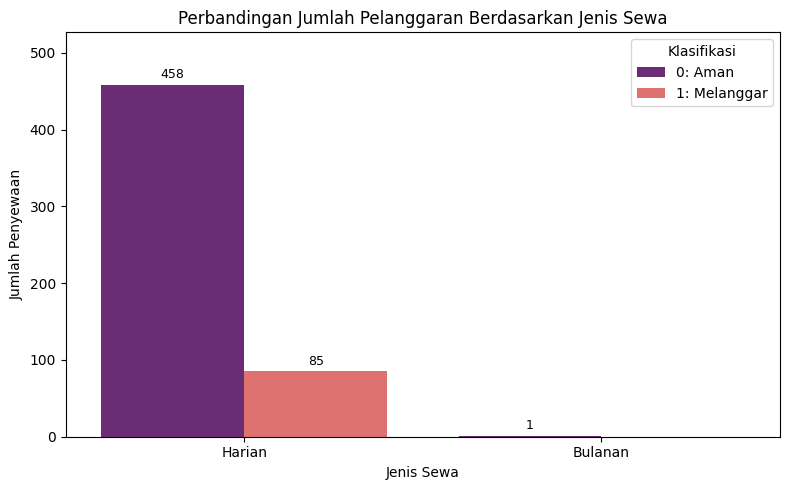
\includegraphics[width=\textwidth]{Gambar/Perbandingan_Jenis_Sewa_Riil.png}
            \caption{Data Riil}
            \label{fig:jenis_sewa_riil}
        \end{subfigure}
        \caption{Perbandingan Jumlah Pelanggaran Berdasarkan Jenis Sewa}
        \label{fig:jenis_sewa}
    \end{figure}
    
    Pada atribut demografis status pernikahan (Gambar~\ref{fig:status_pasutri}) menunjukkan pola yang sama dengan data sintetis, di mana pelanggaran pada data riil tersebar secara ekuivalen (masing-masing tepat 44 kasus) pada kelompok Menikah dan Belum Menikah. Sementara itu, pada status kewarganegaraan (Gambar~\ref{fig:status_kewarganegaraan}), keseluruhan data operasional riil murni diisi oleh WNI, yang mana meniadakan distribusi risiko pada WNA seperti yang sebelumnya disimulasikan pada data sintetis.
    
    \begin{figure}[H]
        \centering
        \begin{subfigure}[b]{0.45\textwidth}
            \centering
            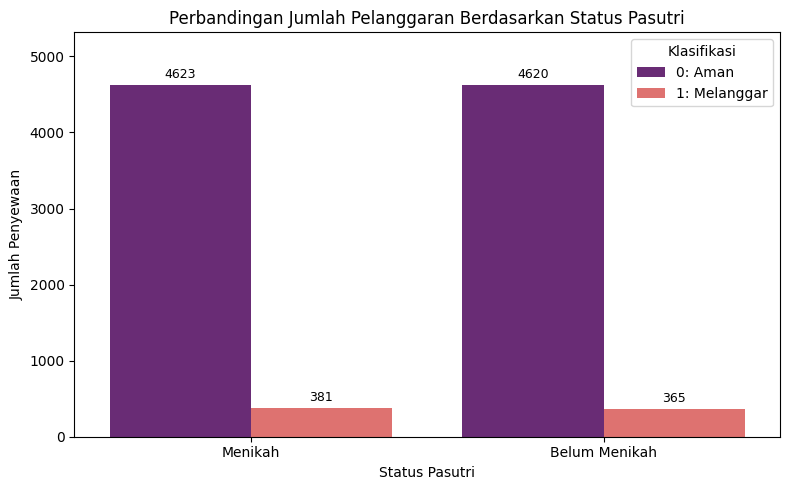
\includegraphics[width=\textwidth]{Gambar/Perbandingan_Status_Pasutri_Dummy.png}
            \caption{Data Sintetis (\textit{Dummy})}
            \label{fig:status_pasutri_dummy}
        \end{subfigure}
        \hfill
        \begin{subfigure}[b]{0.45\textwidth}
            \centering
            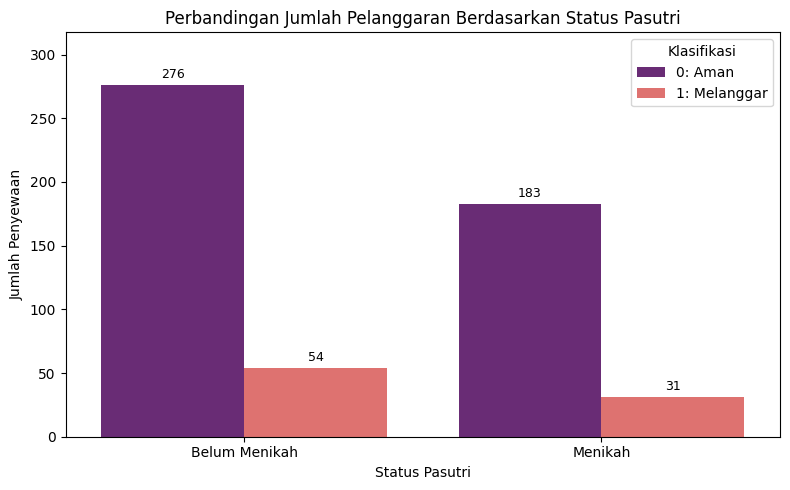
\includegraphics[width=\textwidth]{Gambar/Perbandingan_Status_Pasutri_Riil.png}
            \caption{Data Riil}
            \label{fig:status_pasutri_riil}
        \end{subfigure}
        \caption{Perbandingan Jumlah Pelanggaran Berdasarkan Status Pasutri}
        \label{fig:status_pasutri}
    \end{figure}

    \begin{figure}[H]
        \centering
        \begin{subfigure}[b]{0.45\textwidth}
            \centering
            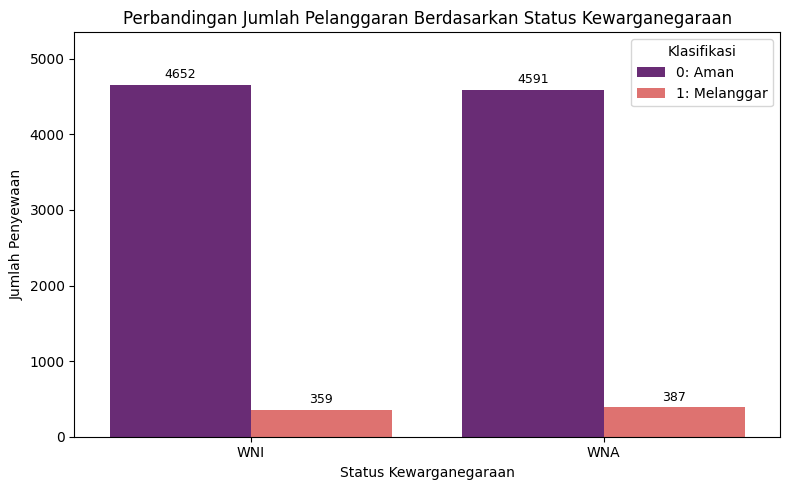
\includegraphics[width=\textwidth]{Gambar/Perbandingan_Status_Kewarganegaraan_Dummy.png}
            \caption{Data Sintetis (\textit{Dummy})}
            \label{fig:status_kewarganegaraan_dummy}
        \end{subfigure}
        \hfill
        \begin{subfigure}[b]{0.45\textwidth}
            \centering
            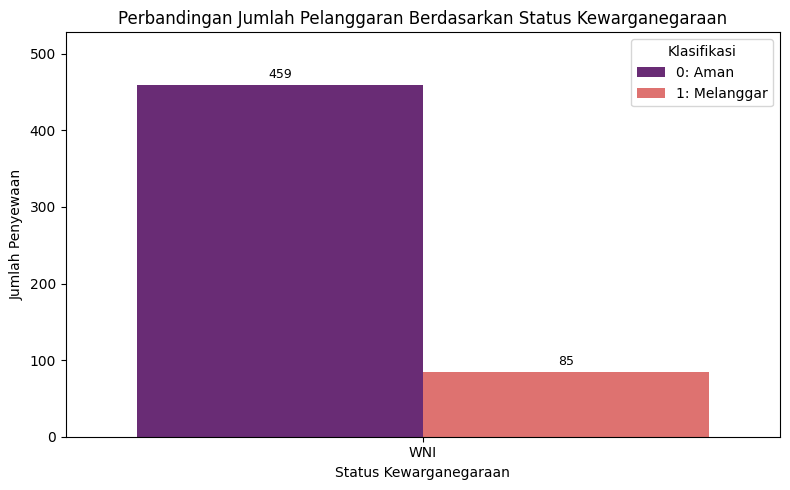
\includegraphics[width=\textwidth]{Gambar/Perbandingan_Status_Kewarganegaraan_Riil.png}
            \caption{Data Riil}
            \label{fig:status_kewarganegaraan_riil}
        \end{subfigure}
        \caption{Perbandingan Jumlah Pelanggaran Berdasarkan Status Kewarganegaraan}
        \label{fig:status_kewarganegaraan}
    \end{figure}

    Terakhir, visualisasi metode pembayaran terlihat pada Gambar~\ref{fig:metode_pembayaran}. Berbeda dengan data sintetis yang mengasumsikan distribusi merata, data riil memperlihatkan bahwa pelanggaran paling banyak tercatat pada transaksi digital seperti \textit{Others} (36 kasus) dan QRIS (27 kasus), disusul oleh transaksi Tunai/\textit{Cash} (20 kasus). Penggunaan kartu kredit dan debit justru terbukti memiliki risiko pelanggaran yang sangat minim di lapangan. Pada rancangan data sintetis, opsi \textit{Others} diasumsikan memiliki variansi yang tinggi dan tersebar secara hampir merata pada berbagai macam platform digital kekinian (seperti Paylater, Ovo, Shopeepay, Gopay, hingga Crypto) dengan rentang 275 hingga 297 transaksi per metode. Namun, fakta pada operasional data riil menunjukkan bahwa kategori \textit{Others} justru secara mutlak didominasi oleh metode konvensional berupa ``Transfer'' (227 transaksi), sementara sisanya menggunakan metode ``Aplikasi'' yang hanya tercatat sebanyak 1 transaksi. Temuan ini membuktikan bahwa pada praktiknya di lapangan, opsi pembayaran alternatif penyewa nyatanya tidak bervariasi dan hanya terpusat pada metode transfer bank.

    \begin{figure}[H]
        \centering
        \begin{subfigure}[b]{0.45\textwidth}
            \centering
            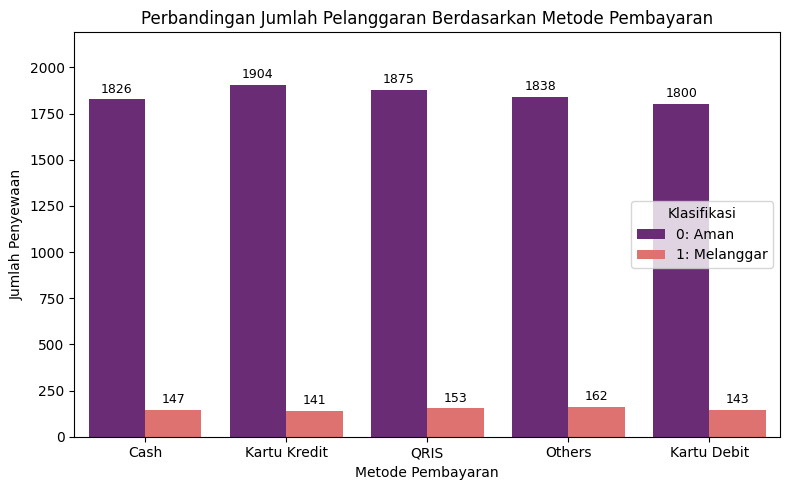
\includegraphics[width=\textwidth]{Gambar/Perbandingan_Metode_Pembayaran_Dummy.png}
            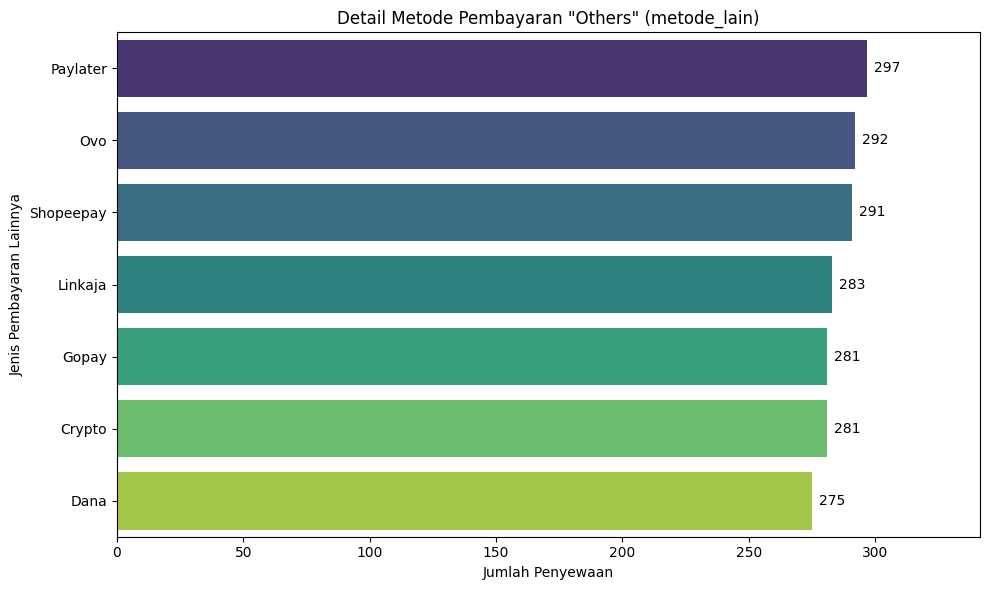
\includegraphics[width=\textwidth]{Gambar/Detail_Others_Dummy.png}
            \caption{Data Sintetis (\textit{Dummy})}
            \label{fig:metode_pembayaran_dummy}
        \end{subfigure}
        \hfill
        \begin{subfigure}[b]{0.45\textwidth}
            \centering
            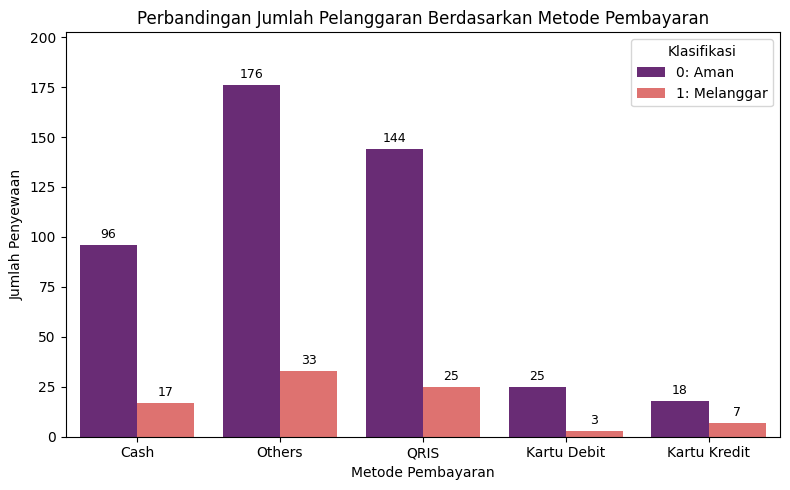
\includegraphics[width=\textwidth]{Gambar/Perbandingan_Metode_Pembayaran_Riil.png}
            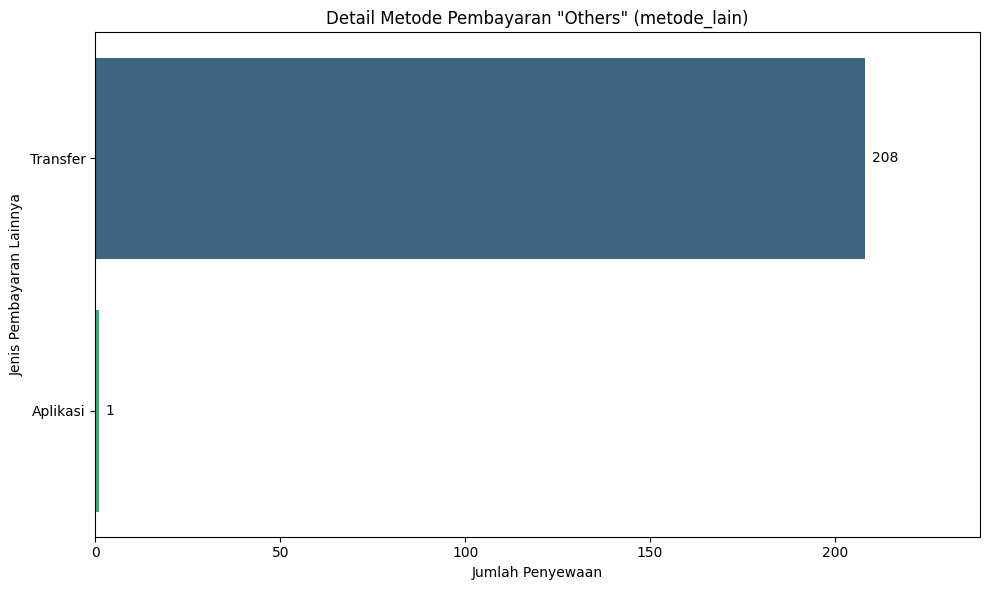
\includegraphics[width=\textwidth]{Gambar/Detail_Others_Riil.png}
            \caption{Data Riil}
            \label{fig:metode_pembayaran_riil}
        \end{subfigure}
        \caption{Perbandingan Jumlah Pelanggaran Berdasarkan Metode Pembayaran}
        \label{fig:metode_pembayaran}
    \end{figure}
\end{enumerate}